\section{Reading Notes of \texorpdfstring{\cite{gf}}{Lg}}
\subsection{June 9 Local Structure of Fractals}
\subsubsection{Densities(5.1)}

\begin{definition}[$s$-sets] $ $\\
    Borel sets of Hausdorff dimension $s$ with positive finite s-dimensional Hausdorff measure.
\end{definition}

\begin{definition}[Density of an $s$-set]
    We define the lower and upper densities of an $s$ -set $F$ at a point $x \in \mathbb{R}^{n}$ as
        $$
        \underline{D}^{s}(F, x)=\varliminf_{r \rightarrow 0} \frac{\mathcal{H}^{s}(F \cap B(x, r))}{(2 r)^{s}}
        $$
    and
        $$
        \bar{D}^s(F, x)=\varlimsup_{r \rightarrow 0} \frac{\mathcal{H}^{s}(F \cap B(x, r))}{(2 r)^{s}}
        $$
    respectively (note that $|B(x, r)|=2 r)$. If $\underline{D}^{s}(F, x)=\bar{D}^{s}(F, x)$, we say that the density of $F$ at $x$ exists and we write $D^{s}(F, x)$ for the common value.
\end{definition}

\begin{definition}[Regular Point]
    A regular point $x$ of $F$ is a point at which $$\underline{D}^s(F, x) = \overline{D}^s(F, x) = 1$$
    otherwise, $x$ is an irregular point. 
\end{definition}

\begin{definition}[Regular of $s$-set]
    An $s$-set is termed regular if $\mathcal{H}^{s}$-almost all of its points (i.e. all of its points except for a set of $\mathcal{H}^{s}-$measure 0) are regular and irregular if $\mathcal{H}^{s}$-almost all of its points are irregular.
\end{definition}

\textbf{Note: }\begin{enumerate}
    \item 'irregular' does not mean 'not regular'
    \item $s$-set $F$ must be irregular unless $s$ is an integers
    \item a regular 1-set consists of portions of rectifiable curves of finite length, whereas an irregular 1-set is totally disconnected and dust-like and typically of fractalform.
\end{enumerate}


\begin{proposition}\label{prop4.9}
    Let $\mu$ be a mass distribution on $\mathbb{R}^{n}$, let $F \subset \mathbb{R}^{n}$ be a Borel set and let $0<c<\infty$ be a constant.
    \begin{enumerate}[a.]
        \item\label{prop4.9a}  If $\varlimsup_{r \rightarrow 0} \mu(B(x, r)) / r^{s}<c$ for all $x \in F$, then $\mathcal{H}^{s}(F) \geq \mu(F) / c$.
        \item\label{prop4.9b} If $\uplim_{r \rightarrow 0} \mu(B(x, r)) / r^{s}>c \text { for all } x \in F, \text { then } \mathcal{H}^{s}(F) \leq 2^{s} \mu\left(\mathbb{R}^{n}\right) / c$
    \end{enumerate}
\end{proposition}

\begin{proposition}\label{prop5.1}
    Let $F$ be an $s$-set in $\mathbb{R}^{n}$. Then
    \begin{enumerate}[a.]
        \item $\underline{D}^{s}(F, x)=\bar{D}^{s}(F, x)=0$ for $\mathcal{H}^{s}$-almost all $x \notin F$
        \item $2^{-s} \leq \bar{D}^{s}(F, x) \leq 1$ for $\mathcal{H}^{s}$-almost all $x \in F$.
    \end{enumerate}
\end{proposition}
\textbf{\textit{Partial Proof: }}\begin{enumerate}[a.]
    \item If $F$ is closed and $x \notin F$, then $B(x, r) \cap F=\emptyset$ if $r$ is small enough. Hence, $\lim _{r \rightarrow 0} \mathcal{H}^{s}(F \cap B(x, r)) /(2 r)^{s}=0$. If $F$ is not closed, the proof is a little more involved and we omit it here.
    \item This follows quickly from Proposition \ref{prop4.9} \ref{prop4.9a} by taking $\mu$ as the restriction of $\mathcal{H}^{s}$ to $F$, that is, $\mu(A)=\mathcal{H}^{s}(F \cap A):$ if
    $$
    F_{1}=\left\{x \in F: \bar{D}^{s}(F, x)=\varlimsup_{r \rightarrow 0} \frac{\mathcal{H}^{s}(F \cap B(x, r))}{(2 r)^{s}}<2^{-s} c\right\},
    $$
    then $\mathcal{H}^{s}\left(F_{1}\right) \geq \mathcal{H}^{s}(F) / c \geq \mathcal{H}^{s}\left(F_{1}\right) / c$. If $0<c<1$, this is only
    possible if $\mathcal{H}^{s}\left(F_{1}\right)=0$; thus, for almost all $x \in F$, we have $\bar{D}^{s}(F, x) \geq 2^{-s}$. The upper bound follows in essentially the same way using Proposition \ref{prop4.9} \ref{prop4.9b}.
\end{enumerate}

\begin{proposition}\label{5.4}
    Let $F$ be an $s$-set and let $E$ be a Borel set of $F$, then:
    $$
\frac{\mathcal{H}^{s}(F \cap B(x, r))}{(2 r)^{s}}=\frac{\mathcal{H}^{s}(E \cap B(x, r))}{(2 r)^{s}}+\frac{\mathcal{H}^{s}((F \backslash E) \cap B(x, r))}{(2 r)^{s}}
$$
for almost all $x$ in $E$, we have
$$
\frac{\mathcal{H}^{s}((F \backslash E) \cap B(x, r))}{(2 r)^{s}} \rightarrow 0 \quad \text { as } r \rightarrow 0
$$
by Proposition \ref{prop5.1} a., so letting $r \rightarrow 0$ gives
$$
\underline{D}^{s}(F, x)=\underline{D}^{s}(E, x) ; \quad \bar{D}^{s}(F, x)=\bar{D}^{s}(E, x)
$$
for $\mathcal{H}^s$-almost all $x$ in $E$.
\end{proposition} 
\textbf{Note: } 
\begin{enumerate}[(i)]
    \item if $E$ is a subset of an $s-$set $F$ with $\mathcal{H}^s(E)>0$, then $E$ is regular if $F$ is regular and vice versa. 
    \item intersection of a regular and an irrgular set has $\HH^s$-measuer zero. 
\end{enumerate}

\begin{theorem}
    Let $F$ be an s-set in $\RR^2$. Then $F$ is irregular unless $s$ is an integer.
\end{theorem}

\newpage
\subsubsection{Structure of 1-sets(5.2)}
\begin{theorem}[Decomposition Theorem]
    Let $F$ be a 1 -set. The set of regular points of $F$ forms a regular set, the set of irregular points forms an irregular set.
\end{theorem}
\proof: By Proposition \ref{5.4} taking $E$ as the set of regular and irregular points. 

\begin{figure}[H]
    \centering
    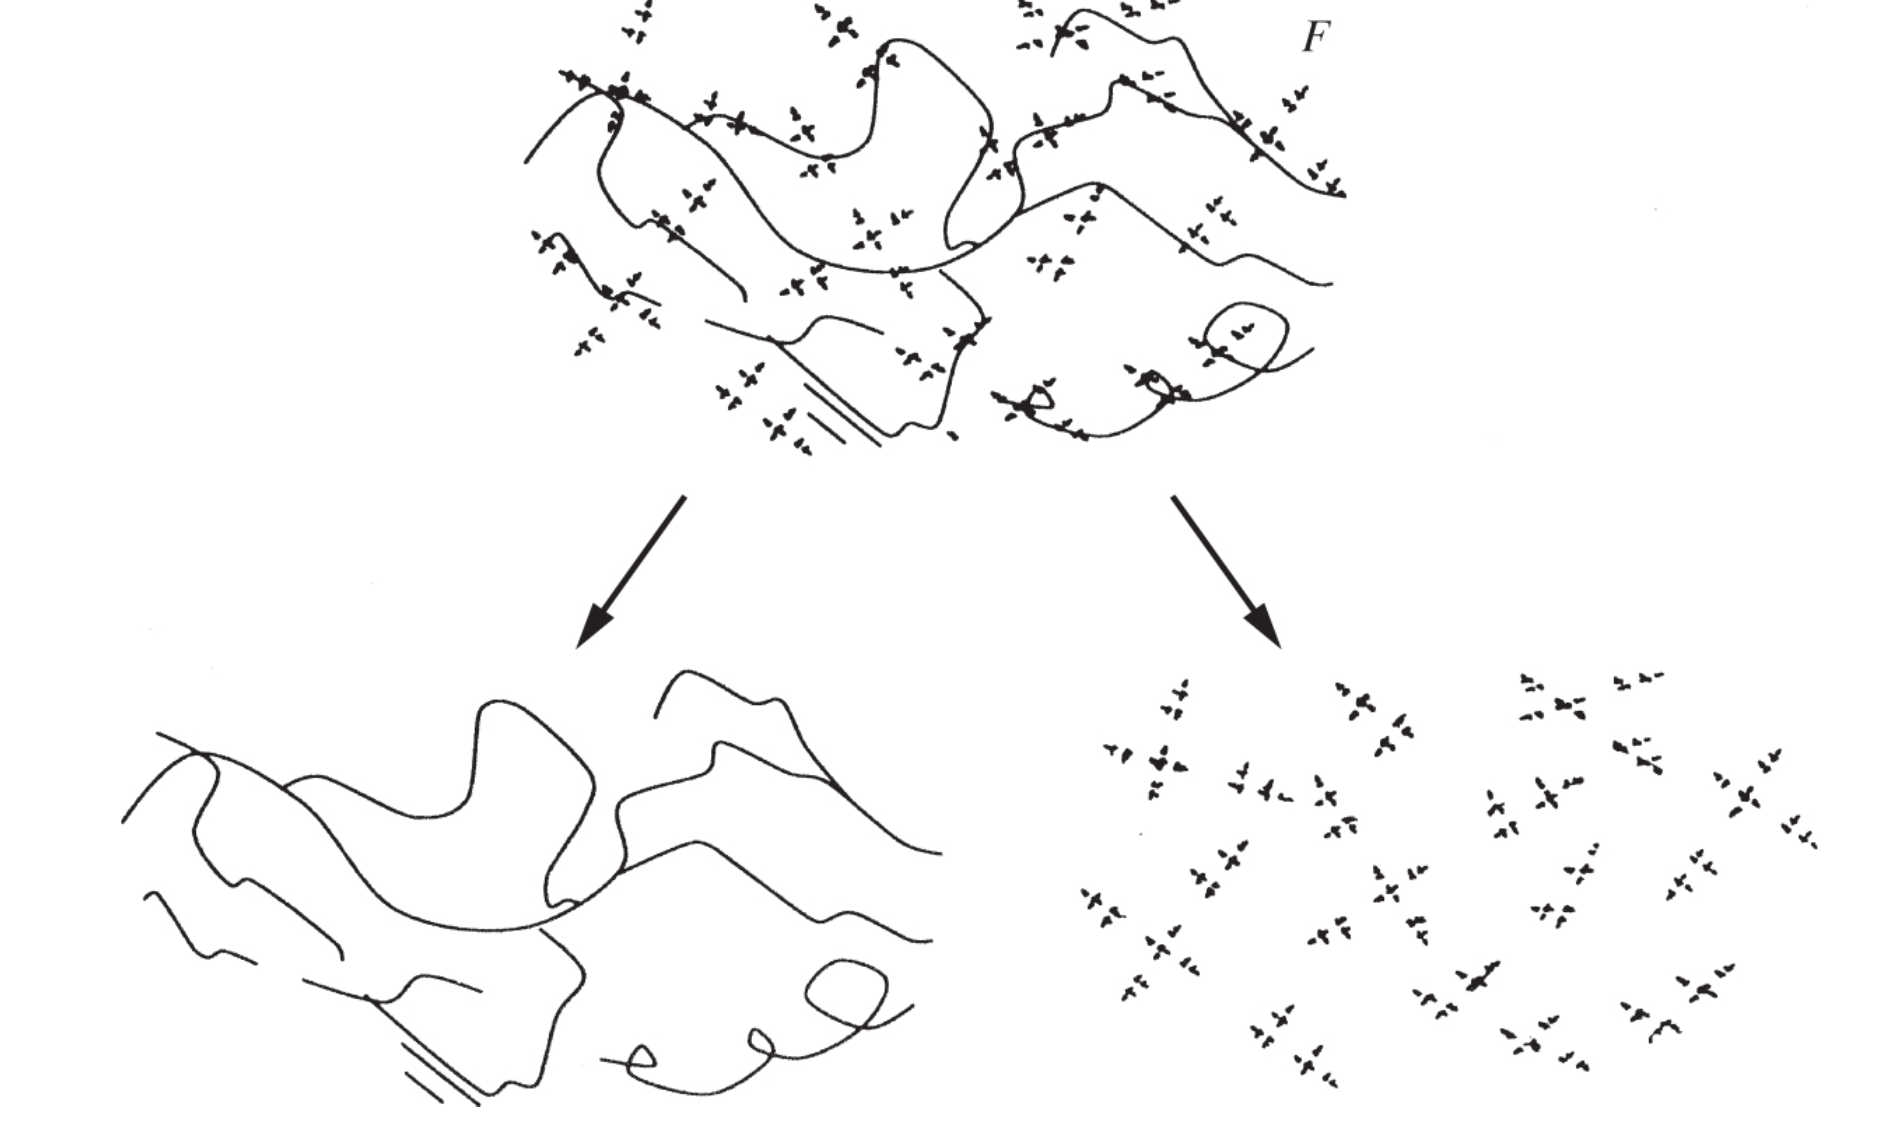
\includegraphics[width=.66\textwidth]{images/decomp1set.png}
    \caption{Decomposition of a 1-set into a regular ‘curve-like’ part and an irregular ‘curve-free’ part}
    \label{fig:decomp1set}
\end{figure}

\textbf{Note: }Regular 1-sets are made up from \textit{pieces of curve}, whereas irregular 1-sets are dust- like and \textit{‘curve-free’}, that is, intersect any (finite length) curve in length zero, illustrated in Figure \ref{fig:decomp1set}.

\begin{definition}[Curve(Jordan Curve)]
    A Jordan curve C is the image of a continuous injection(one-to-one) $\psi:[a,b]\rightarrow\RR^2$, where $[a, b]\subset \RR$ is a proper closed interval. 
\end{definition}

\textit{Length}: 
$$
\LL(C) = \sup \sum_{i=1}^\infty |x_i - x_{i-1}|
$$
where the supremum is taken over all dissections of $C$ by points $x_0, x_1, \dots, x_m$ in that order along the curve. 

\begin{definition}[Rectifiable Curve]
    If $\LL(C)$ is positive and finite, $C$ is a rectifiable curve. 
\end{definition}

\begin{lemma}\label{lemma5.4}
    If $C$ is a rectifiable curve, then $\HH^1(C) = \LL(C)$
\end{lemma}
\proof:
For $x, y \in C$, let $C_{x, y}$ denote that part of $C$ between $x$ and $y$. As orthogonal projection onto the line through $x$ and $y$ does not increase distances, Proposition \ref{Haus-holder} gives $\mathcal{H}^{1}\left(C_{x, y}\right) \geq \mathcal{H}^{1}[x, y]=|x-y|$, where $[x, y]$ is the straight-line segment joining $x$ to $y$. Hence, for any dissection $x_{0}, x_{1}, \ldots, x_{m}$ of $C$
$$
\sum_{i=1}^{m}\left|x_{i}-x_{i-1}\right| \leq \sum_{i=1}^{m} \mathcal{H}^{1}\left(C_{x_{i}, x_{i-1}}\right) \leq \mathcal{H}^{1}(C)
$$
so taking the supremum over all dissections gives $\mathcal{L}(C) \leq \mathcal{H}^{\prime}(C)$. On the other hand, let $f:[0, \mathcal{L}(C)] \rightarrow C$ be the mapping that takes to the point on $C$ at distance $t$ along the curve from one of its ends. Clearly, $|f(t)-f(u)| \leq|t-u|$ for $0 \leq t, u \leq \mathcal{L}(C)$, that is, $f$ is Lipschitz with $\mathcal{H}^{1}(C) \leq \mathcal{H}^{1}[0, \mathcal{L}(C)]=\mathcal{L}(C)$ by Proposition \ref{Haus-holder} as required.

\begin{lemma}\label{lemma5.5}
    A rectifiable curve is a regular 1-set. 
\end{lemma}
\proof: As $C$ is rectifiable $\mathcal{L}(C)<\infty$, and because $C$ has distinct end points $p$ and $q$, it is clear that $\mathcal{L}(C) \geq|p-q|>0$. By Lemma \ref{lemma5.4}, $0<\mathcal{H}^{1}(C)<\infty$, so $C$ is a 1-set.

A point $x$ of $C$ that is not an end point divides $C$ into two parts $C_{p, x}$ and $C_{x, q} .$ If $r$ is sufficiently small, then moving away from $x$ along the curve $C_{x, q}$, we reach a first point $y$ on $C$ with $|x-y|=r$. Then $C_{x, v} \subset B(x, r)$ and
$$
r=|x-y| \leq \mathcal{L}\left(C_{x, y}\right)=\mathcal{H}^{1}\left(C_{x, y}\right) \leq \mathcal{H}^{1}\left(C_{x, q} \cap B(x, r)\right) .
$$
Similarly, $r \leq \mathcal{H}^{1}\left(C_{p, x} \cap B(x, r)\right)$, so, adding, $2 r \leq \mathcal{H}^{1}(C \cap B(x, r))$, if $r$ is
small enough. Thus
$$
\underline{D}^{1}(C, x)=\lim _{r \rightarrow 0} \frac{\mathcal{H}^{1}(C \cap B(x, r))}{2 r} \geq 1 .
$$
By Proposition \ref{prop5.1}(a) $\underline{D}^{1}(C, x) \leq \bar{D}^{1}(C, x) \leq 1$ for $\mathcal{H}^{1}$ -almost all $x$, so
$D^{1}(C, x)$ exists and equals 1 for almost all $x \in C$, so $C$ is regular.

\begin{proposition}\label{prop5.6}
    A curve like 1-set is a regular 1-set. 
\end{proposition}
\proof: If $F$ is a curve-like 1 -set, then $F \subset \bigcup_{i=1}^{\infty} C_{i}$ where the $C_{i}$ are rectifiable curves. For each $i$ and $\mathcal{H}^{1}$ -almost all $x \in F \cap C_{i}$, we have, using Lemma \ref{lemma5.5} and \ref{lemma5.4},
$$
1=\underline{D}^{1}\left(C_{i}, x\right)=\underline{D}^{1}\left(F \cap C_{i}, x\right) \leq \underline{D}^{1}(F, x)
$$
and, hence, $1 \leq \underline{D}^{1}(F, x)$ for almost all $x \in F$. But for almost all $x \in F$, we have $\underline{D}^{1}(F, x) \leq \bar{D}^{1}(F, x) \leq 1$ by Proposition \ref{prop5.1}, so
$D^{1}(F, x)=1$ almost everywhere, and $F$ is regular.


\begin{proposition}Let $F$ be a curve-free 1 -set in $\mathbb{R}^{2}$. Then $\underline{D}^{1}(F, x) \leq \frac{3}{4}$ at almost all $x \in F .$
\end{proposition}

\begin{theorem}\label{thm5.9} $ $
    \begin{enumerate}[a.]
        \item A $1$-set in $\RR^2$ is irregular if and only if it is curve-free.
        \item A 1-set in $\RR^2$ is regular if and only if it is the union of a curve-like set and a set of $\HH^1$-measure zero. 
    \end{enumerate}
\end{theorem}



\newpage
\subsubsection{Tangents to s-sets(5.3)}









\newpage

\subsection{June 7 Hausdorff and packing measures and dimensions}
\subsubsection{Hausdorff Measure(3.1)}
\begin{definition}[Hausdorff Measure]
    Suppose that $F$ is a subset of $\mathbb{R}^n$ and $s\geq 0$. For each $\delta >0$,
    $$
    \mathcal{H}_{\delta}^{s}(F)=\inf \left\{\sum_{i=1}^{\infty}\left|U_{i}\right|^{s}:\left\{U_{i}\right\} \text { is a } \delta \text {-cover of } F\right\} .
    $$
    And we write
    $$
    \mathcal{H}^s (F) = \lim_{\delta\rightarrow 0} \mathcal{H}^s_\delta(F)
    $$
    as the s-dimensional Hausdorff measure on $F$.
\end{definition}

\textbf{Note:}
Thus, we look at all covers of $F$ by sets of diameter at most $\delta$ and seek to minimise the sum of the  $s^{th}$ powers of the diameters.

It can be shown as a measure as: $\mathcal{H}^s(\emptyset) = 0$; if $E$ is contained in $F$, then $\mathcal{H}^s(E)\leq \mathcal{H}^s(F)$; if $\{F_i\}$ is any countable collection of sets, then $\displaystyle \mathcal{H}^{s}\left(\bigcup_{i=1}^{\infty} F_{i}\right) \leq \sum_{i=1}^{\infty} \mathcal{H}^{s}\left(F_{i}\right)$.

\begin{property}[Equivalence of Hausdorff Measure] $ $
    \begin{enumerate}[(i)]
        \item with $n-$dimensional Lebesgue measure: $\mathcal{H}^n(F) = c_n^{-1} \text{vol}^n(F)$ where $c_n$ is the volume of an $n$-dimensional ball of diameter 1, so that $c_{n}=\pi^{n / 2} / 2^{n}(n / 2) !$ if $n$ is even and $c_{n}=\pi^{n / 2} / 2^{n}(n / 2) !$ if odd.
        \item $\mathcal{H}^0(F)$ is the number of points
        \item $\mathcal{H}^1(F)$ is the length of a smooth curve $F$
        \item $\mathcal{H}^2(F) = (4/\pi) \times \operatorname{area}(F)$ if $F$ is a smooth surface
        \item $\mathcal{H}^{3}(F)=(6 / \pi) \times \operatorname{vol}(F)$
        \item $\mathcal{H}^{m}(F)=c_{m}^{-1} \times \operatorname{vol}^{m}(F)$ if $F$ is a smooth $m-$
        dimensional submanifold of $\mathbb{R}^{n}$ (i.e. an $m$-dimensional surface in the classical sense).
    \end{enumerate}
\end{property}

\begin{proposition}[Hölder condition of exponent $\alpha$]\label{Haus-holder}
    Let $F \subset \mathbb{R}^{n}$ and $f: F \rightarrow \mathbb{R}^{m}$ be a mapping such that
$$
|f(x)-f(y)| \leq c|x-y|^{\alpha} \quad(x, y \in F)
$$
for constants $\alpha>0$ and $c>0 .$ Then for each $s$
$$
\mathcal{H}^{s / \alpha}(f(F)) \leq c^{s / \alpha} \mathcal{H}^{s}(F)
$$
In particular, if $f$ is a Lipschitz mapping, that is, if $\alpha=1$, then
$$
\mathcal{H}^{s}(f(F)) \leq c^{s} \mathcal{H}^{s}(F)
$$
\end{proposition}

\textbf{\textit{Proof:}} If $\left\{U_{i}\right\}$ is a $\delta$-cover of $F$, 
then since $\left|f\left(F \cap U_{i}\right)\right| \leq c\left|F \cap U_{i}\right|^{\alpha} \leq c\left|U_{i}\right|^{a}$, 
it follows that $\left\{f\left(F \cap U_{i}\right)\right\}$ is a $c \delta^{a}$-cover of $f(F)$. 
Thus, $\displaystyle\sum_{i}\left|f\left(F \cap U_{i}\right)\right|^{s / \alpha} \leq c^{s / \alpha} \sum_{i}\left|U_{i}\right|^{s}$, so that $\mathcal{H}_{c \delta^{\prime}}^{s / \alpha}(f(F)) \leq c^{s / \alpha} \mathcal{H}_{\delta}^{s}(F)$. Letting
$\delta \rightarrow 0$ gives the result. 
The result for the Lipschitz case is immediate on setting $\alpha=1$.

\begin{property}[Scaling Property]
    Let $f: \mathbb{R}^{n} \rightarrow \mathbb{R}^{n}$ be a similarity transformation of scale factor $\lambda>0$. If $F \subset \mathbb{R}^{n}$, then
$$
\mathcal{H}^{s}(f(F))=\lambda^{s} \mathcal{H}^{s}(F)
$$
\end{property}

\textbf{\textit{Proof:}} $|f(x)-f(y)|=\lambda|x-y|$ and so $\left|f^{-1}(x)-f^{-1}(y)\right|=\lambda^{-1}|x-y| \quad(x, y \in F)$ and apply Proposition \ref{Haus-holder} for $c=\lambda$.

\textbf{Note: } property above can be considered as scaling of a length, area, or a volume by mutiplying $\lambda, \lambda^2, \lambda^3$ respectively. And if $f$ is congruence or isometry, that is, $|f(x)-f(y)| = |x-y|$, then $\mathcal{H}^s(f(F)) = \mathcal{H}^s(F)$. 
Thus, Hausdorff measures are \textit{translation invarient}(i.e. $\mathcal{H}^s(F+z) = \mathcal{H}^s(F)$ where $F+z = \{x+z:x\in F\}$) and \textit{rotation invariant}. 

\newpage
\subsubsection{Hausdorff dimension(3.2)}

\begin{property}[$\mathcal{H}^s(F)$ is non-increasing]
    If $t<s$ and $\{U_i\}$ is a $\delta$ cover of $F$, then
    $$
    \sum_{i}\left|U_{i}\right|^{t} \leq \sum_{i}\left|U_{i}\right|^{\mid-s}\left|U_{i}\right|^{s} \leq  \sum_{i}\left|U_{i}\right|^{s}\delta^{t-s} = \delta^{t-s} \sum_{i}\left|U_{i}\right|^{s}
    $$
    taking infima over all $\delta$-covers,
    $$
    \mathcal{H}^t_\delta(F)\leq \delta^{t-s}\mathcal{H}^s_\delta(F)
    $$
    which is non-increasing when $\delta\leq 1$.
\end{property}

\begin{definition}[Hausdorff Dimension]
    $$\operatorname{dim}_{\mathrm{H}} F=\inf \left\{s \geq 0: \mathcal{H}^{s}(F)=0\right\}=\sup \left\{s: \mathcal{H}^{s}(F)=\infty\right\}$$
(taking the supremum of the empty set to be o), so that
$$
\mathcal{H}^{s}(F)=\left\{\begin{array}{ll}
\infty & \text { if } 0 \leq s<\operatorname{dim}_{\mathrm{H}} F \\
0 & \text { if } s>\operatorname{dim}_{\mathrm{H}} F
\end{array}\right.
$$
If $s=\operatorname{dim}_{\mathrm{H}} F$, then $\mathcal{H}^{s}(F)$ may be zero or infinite or may satisfy
$$
0<\mathcal{H}^{s}(F)<\infty .
$$
\end{definition}

\textbf{Note: }Conisder that when $\delta\rightarrow 0$, if $\mathcal{H}^s<\infty$ then $\mathcal{H}^t(F) = 0$ for $t>s$, s.t. there is a critical value of $s$ at which measure "jumps" from $\infty$ to $0$, named \textit{Hausdorff dimension}.



\begin{proposition}[Hausdorff Dimension under Lipschitz Mapping]\label{H-under-L} $ $
    \begin{enumerate}[a.]
        \item Let $F \subset \mathbb{R}^{n}$ and suppose that $f: F \rightarrow \mathbb{R}^{m}$ satisfies the Hölder condition
$$
|f(x)-f(y)| \leq c|x-y|^{\alpha} \quad(x, y \in F) .
$$
Then $\operatorname{dim}_{\mathrm{H}} f(F) \leq(1 / \alpha) \operatorname{dim}_{\mathrm{H}} F .$ In particular, if $f$ is a Lipschitz
mapping, that is, if $\alpha=1$, then $\operatorname{dim}_{H} f(F) \leq \operatorname{dim}_{H} F$.
\item If $f: F \rightarrow \mathbb{R}^{m}$ is a bi-Lipschitz transformation, that is,
$$
c_{1}|x-y| \leq|f(x)-f(y)| \leq c|x-y| \quad(x, y \in F),
$$
where $0<c_{1} \leq c<\infty$, then $\operatorname{dim}_{\mathrm{H}} f(F)=\operatorname{dim}_{\mathrm{H}} F$.
    \end{enumerate}
\end{proposition}

\newpage

\subsection{June 2-3 Box-Counting Dimension}
\subsubsection{Box-Counting Dimensions(2.1)}

\begin{definition}[$\delta$-mesh]
    The family of cubes of the form
$$
\left[m_{1} \delta,\left(m_{1}+1\right) \delta\right] \times \cdots \times\left[m_{n} \delta,\left(m_{n}+1\right) \delta\right],
$$
where $m_{1}, \ldots, m_{n}$ are integers, is called the $\delta$-mesh or $\delta$-grid of $\mathbb{R}^n$.
\end{definition}

\begin{definition}[Diameter]
    any subset of $n-$dimensional Euclidean space, $\mathbb{R}^n$, the \textbf{diameter} of $U$ is defined as $|U|=\sup \{|x-y|:x, y\in U\}$
\end{definition}

\begin{definition}[Box-Counting Dimension]\label{bcd-def}
    The lower and upper box-counting dimensions of a subset $F$ of $\mathbb{R}^{n}$ are given by
    $$\underline{\operatorname{dim}_{\mathrm{B}}} F=\varliminf_{\delta \rightarrow 0} \frac{\log N_{\delta}(F)}{-\log \delta}$$
    $$\overline{\operatorname{dim}}_{\mathrm{B}} F=\varlimsup_{\delta \rightarrow 0} \frac{\log N_{\delta}(F)}{-\log \delta}$$
    
and the box-counting dimension of $F$ by
$$
\operatorname{dim}_{\mathrm{B}} F=\lim _{\delta \rightarrow 0} \frac{\log N_{\delta}(F)}{-\log \delta}
$$
(if this limit exists), where $N_{\delta}(F)$ is any of the following:
\begin{enumerate}[i]
    \item the smallest number of sets of diameter at most $\delta$ that cover $F$
    \item  the smallest number of closed balls of radius $\delta$ that cover $F$
    \item  the smallest number of cubes of side $\delta$ that cover $F$;
    \item  the number of $\delta$-mesh cubes that intersect $F$;
    \item  the largest number of disjoint balls of radius $\delta$ with centres in $F$  
\end{enumerate}  
Figure \ref{fig:bcd-def-vis} illustrates Five ways of finding the box dimension of $F$.

\end{definition}


\begin{figure}[t]
    \centering
    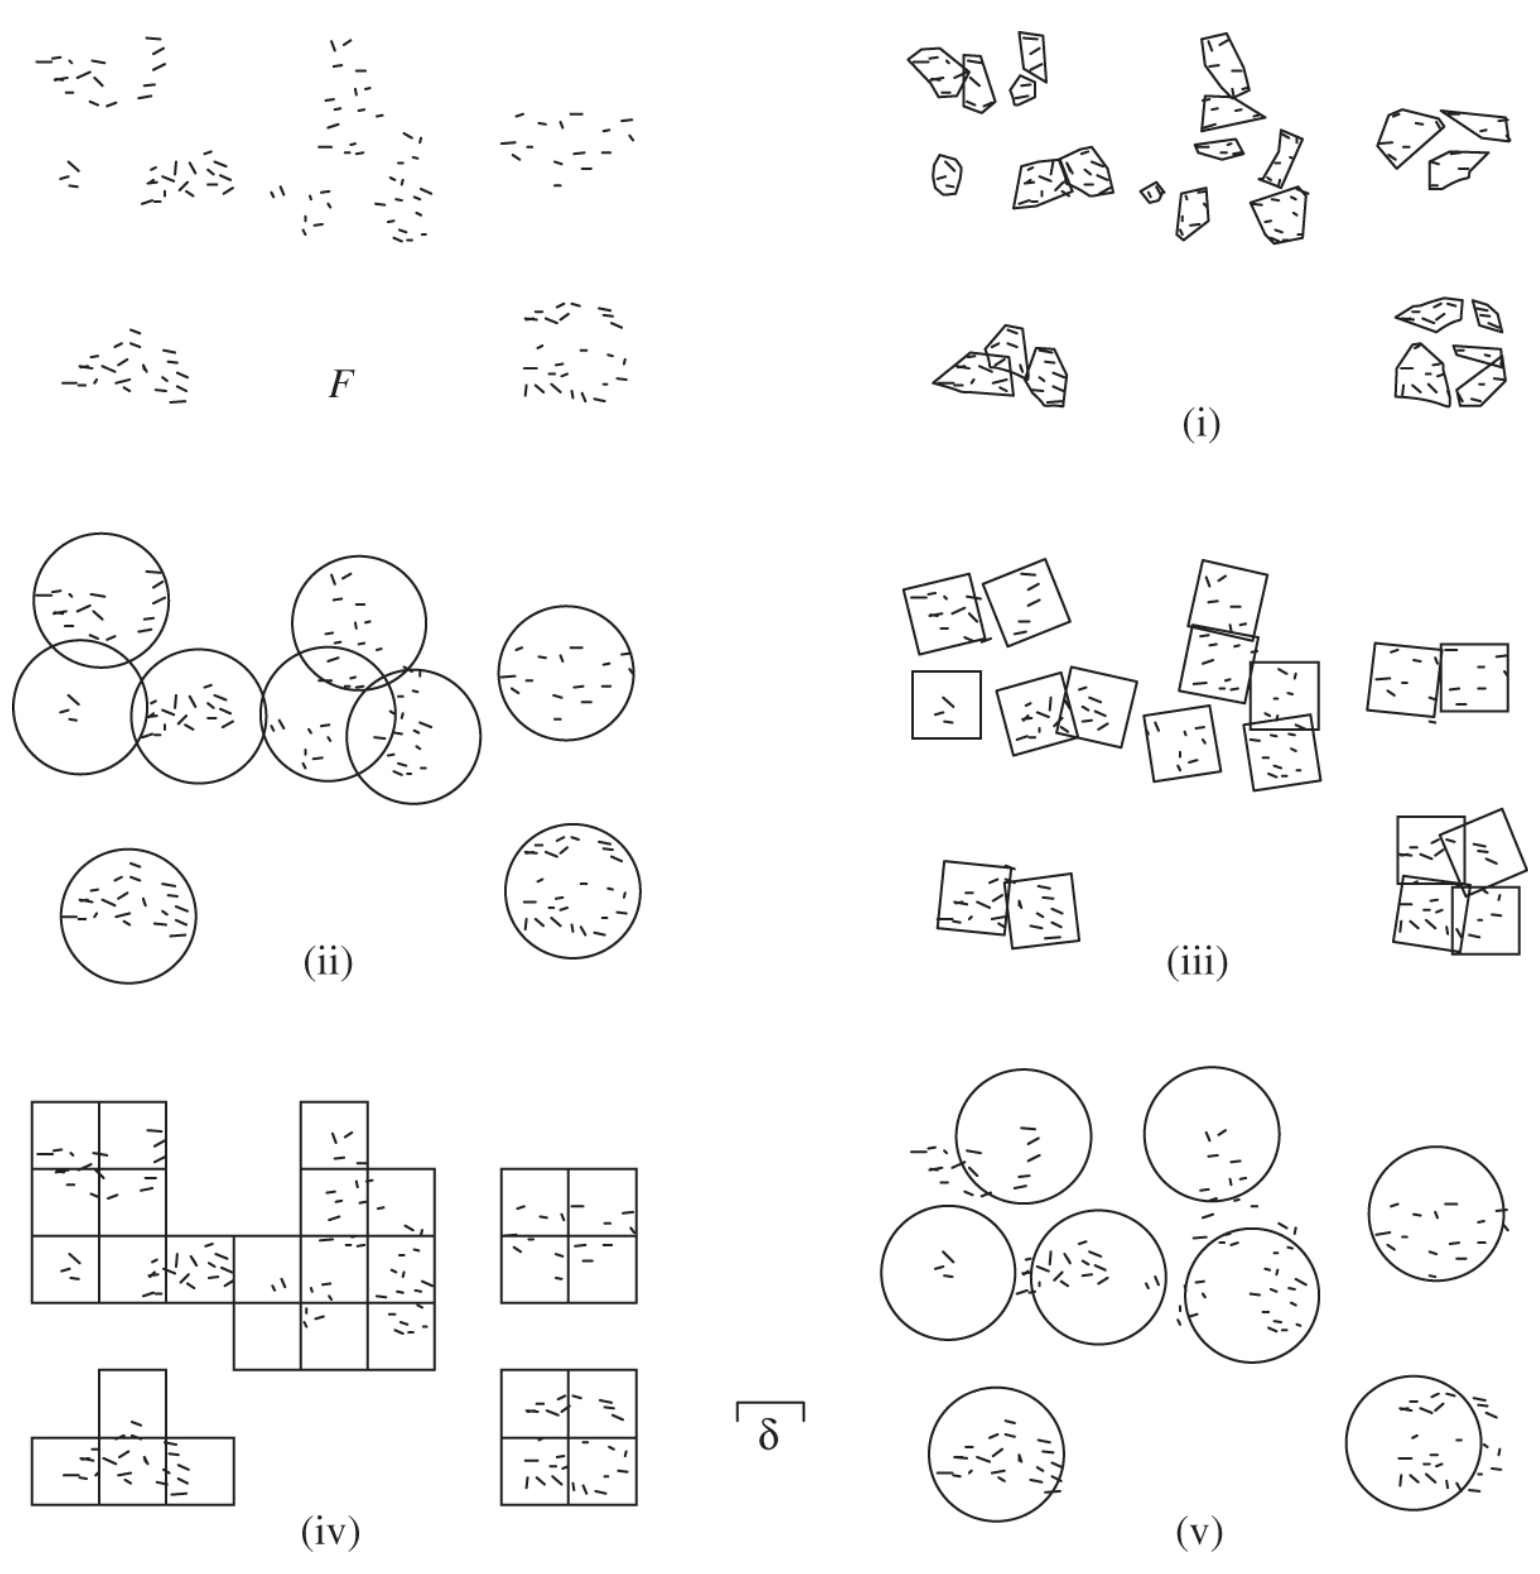
\includegraphics[width=.66\textwidth]{images/bcd-def-vis.png}
    \caption{Five ways of finding the box dimension of $F$}
    \label{fig:bcd-def-vis}
\end{figure}


\textbf{Motivation:}
If $N_\delta(F)$ obeys, at least approximately, a power law
$$N_{\delta}(F) \simeq c \delta^{-s}$$
for positive constant $c$ and $s$, we say that $F$ has box dimension $s$.
\\
Algorithms to solve for $s$:
$$
\log N_{\delta}(F) \simeq \log c-s \log \delta
$$
so
$$
s \simeq \frac{\log N_{\delta}(F)}{-\log \delta}+\frac{\log c}{\log \delta}
$$
and we might hope to obtain $s$ as
$$
s=\lim _{\delta \rightarrow 0} \frac{\log N_{\delta}(F)}{-\log \delta},
$$
with the second term disapperaing in the limit. And this implies that we assume that $\delta$ is sufficiently small. 


Roughly speaking, equation for dimension says that $N_{\delta}(F) \simeq c \delta^{-s}$ for small $\delta$, where $s=\operatorname{dim}_{\mathrm{B}} F$, or, more precisely, that
$$
N_{\delta}(F) \delta^{s} \rightarrow \infty \quad \text { if } s<\operatorname{dim}_{\mathrm{B}} F
$$
and
$$
N_{\delta}(F) \delta^{s} \rightarrow 0 \quad \text { if } s>\operatorname{dim}_{\mathrm{B}} F .
$$

\textbf{Proof of Equivalence of Definition \ref{bcd-def}}:\\
e.g.: (i)$\Leftrightarrow$(iv): Let $N_\delta(F)$ for the smallest number of sets of diameter $\delta$ that can cover $F$ whereas $N_\delta^\prime(F)$ be the number of $\delta$-mesh cubes that intersect $F$. 
Note that these cubes provide a collection of $N_\delta^\prime(F)$ sets of diameter $\delta\sqrt{n}$(diagonal for "diameter at most $\delta$") that cover $F$, $$N_{\delta\sqrt{n}}(F)\leq N_\delta^\prime(F)$$
On the other hand, set of diameter at most $\delta$ is(or must be) contained in $3^n$ mesh cubes of side $\delta$(e.g. choosing a cube containing some points of the set with its all neighbouring cubes, like the middle one and its 8 neighnors when $n=2$). Then we have:
$$ N_\delta^\prime(F) \leq 3^n N_\delta(F)$$
Combining these inequalities and dividing by $-\log \delta$,
$$
\frac{\log N_{\delta \sqrt{n}}(F)}{-\log (\delta \sqrt{n})+\log \sqrt{n}} \leq \frac{\log N_{\delta}^{\prime}(F)}{-\log \delta} \leq \frac{\log 3^{n}+\log N_{\delta}(F)}{-\log \delta}
$$
so taking lower limits as $\delta \rightarrow 0$,
$$\varliminf_{\delta \rightarrow 0} \frac{\log N_{\delta}(F)}{-\log \delta} \leq \varliminf_{\delta \rightarrow 0} \frac{\log N_{\delta}^{\prime}(F)}{-\log \delta} \leq \varliminf_{\delta \rightarrow 0} \frac{\log N_{\delta}(F)}{-\log \delta}$$
with the other terms diappearing in the limit. Thus, lower limit works as sama as for both $N_\delta(F)$, and similar for upper box dimension. 

\textbf{\textit{\\Calculations}}: See Exercise \ref{calculation}

\textbf{\\Note: }More generally a set $F$ made up of $m$ similar disjoint copies of itself at scale $r$ has $$\operatorname{dim}_{\mathrm{B}} F=\log m /-\log r$$

Consider the neighborhood: $F_{\delta}=\left\{x \in \mathbb{R}^{n}:|x-y| \leq \delta \quad\right.$ for some $\left.y \in F\right\}$. The rate at which the $n$-dimensional volume, that is, $n$-dimensional Lebesgue measure $\mathcal{L}^n$, of $F_\delta$ shrinks as $\delta\rightarrow 0$

This idea extends to fractional dimensions. If $F$ is a subset of $\mathbb{R}^{\prime}$ and $\displaystyle\lim _{\delta \rightarrow 0}\left(\mathcal{L}^{n}\left(F_{\delta}\right) / \delta^{n-s}\right)=c$ for some $s>0$ and $0<c<\infty$, it makes sense to
regard $F$ as $s$ -dimensional, and it turns out that $s$ is just the boxcounting dimension. The number $c$ is called the \textit{$s$-dimensional Minkowski content} of $F$ --- a quantity that is useful in some concepts but has the disadvantages that it does not exist for many standard fractals and that it is not necessarily additive on disjoint subsets, that is, is not a measure. Even if this limit does not exist, we can take lower and upper limits, and these are related to the box dimensions.


\begin{proposition}
    If $F$ is a subset of $\mathbb{R}^{n}$, then
$$
\underline{\operatorname{dim}}_{\mathrm{B}} F=n-\varlimsup_{\delta \rightarrow 0} \frac{\log \mathcal{L}^{n}\left(F_{\delta}\right)}{\log \delta}
$$
$$
\overline{\operatorname{dim}}_{\mathrm{B}} F=n-\lowlim_{\delta \rightarrow 0} \frac{\log \mathcal{L}^{n}\left(F_{\delta}\right)}{\log \delta}
$$
where $F_{\delta}$ is the $\delta$ -neighbourhood of $F$. 
\end{proposition}
\textit{Proof: }
If $F$ can be covered by $N_{\delta}(F)$ balls of radius $\delta<1$, then $F_{\delta}$ can be covered by the concentric balls of radius $2 \delta .$ Hence,
$$
\mathcal{L}^{n}\left(F_{\delta}\right) \leq N_{\delta}(F) c_{n}(2 \delta)^{n},
$$
where $c_{n}$ is the volume of the unit ball in $\mathbb{R}^{n} .$ Taking logarithms,
$$
\frac{\log \mathcal{L}^{n}\left(F_{\delta}\right)}{-\log \delta} \leq \frac{\log 2^{n} c_{n}+n \log \delta+\log N_{\delta}(F)}{-\log \delta}
$$
so
$$
\varliminf_{\delta \rightarrow 0} \frac{\log \mathcal{L}^{n}\left(F_{\delta}\right)}{-\log \delta} \leq -n+\underline{\operatorname{dim}}_{\mathrm{B}} F
$$
with a similar inequality for the upper limits. On the other hand, if there are $N_{\delta}(F)$ disjoint balls of radius $\delta$ with centres in $F$, then by adding their volumes,
$$
N_{\delta}(F) c_{n} \delta^{n} \leq \mathcal{L}^{n}\left(F_{\delta}\right)
$$
Taking logarithms and letting $\delta \rightarrow 0$ gives the opposite inequality to the third inequality, using Equivalent definition $(\mathrm{v})$.


\textbf{\\Note: }In the context of Proposition above, box dimension is sometimes referred to as Minkowski dimension or Minkowski–Bouligand dimension.


\newpage
\subsubsection{Properties and Problems of Box-Counting Dimension(2.2)}



\begin{proposition}\label{prop2.5} $ $
    \begin{enumerate}[a.]
        \item If $F \subset \mathbb{R}^{n}$ and $f: F \rightarrow \mathbb{R}^{m}$ is a Lipschitz transformation, that is,
        $$
        |f(x)-f(y)| \leq c|x-y| \quad(x, y \in F),
        $$
        then $\underline{\operatorname{dim}_{\mathrm{B}}} f(F) \leq \underline{\operatorname{dim}_{\mathrm{B}}} F$ and $\overline{\operatorname{dim}}_{\mathrm{B}} f(F) \leq \overline{\operatorname{dim}}_{\mathrm{B}} F$.
        
        \item If $F \subset \mathbb{R}^{n}$ and $f: F \rightarrow \mathbb{R}^{m}$ is a bi-Lipschitz transformation, that is,
        $$
        c_{1}|x-y| \leq|f(x)-f(y)| \leq c|x-y| \quad(x, y \in F),
        $$
        where $0<c_{1} \leq c<\infty$, then $\underline{\operatorname{dim}_{B}} f(F)=\underline{\operatorname{dim}}_{B} F$ and
        $\overline{\operatorname{dim}}_{\mathrm{B}} f(F)=\overline{\operatorname{dim}}_{\mathrm{B}} F .$
        
    \end{enumerate}
\end{proposition}


\newpage

\subsection{May 27 Mathematical Background}
\subsubsection{Measures and Mass Distributions(1.3)}

\begin{definition}[Measure]\label{measure}
    We call $\mu$ a measure on $\mathbb{R}^{n}$ if $\mu$ assigns a non-negative number, possibly $\infty$, to each subset of $\mathbb{R}^{n}$ such that\\
$
\begin{aligned}
\text { (a) }& \mu(\emptyset)=0 \\
\text { (b) }& \mu(A) \leq \mu(B) \quad \text { if } A \subset B \\
\text { (c) }&\text{if } A_{1}, A_{2}, \ldots \text{ is a countable (or finite) sequence of sets, then }\\
& \mu\left(\bigcup_{i=1}^{\infty} A_{i}\right) \leq \sum_{i=1}^{\infty} \mu\left(A_{i}\right)\\
& \text{ with equality in above, that is }\\
& \mu\left(\bigcup_{i=1}^{\infty} A_{i}\right)=\sum_{i=1}^{\infty} \mu\left(A_{i}\right), \\
&\text{ if the }A_i \text{ are disjoint Borel sets.}
\end{aligned}
$
\end{definition}

Condition (a) says that the \textit{\textbf{empty set has
zero measure}}, condition (b) says \textit{\textbf{'the larger the set, the larger the measure'}} and condition (c) says that if a set is a union of a countable number of pieces (which may overlap), then the sum of the measure of the pieces is at least equal to the measure of the whole. If \textit{\textbf{a set is decomposed into a countable number of disjoint Borel sets}}, then the \textit{\textbf{total measure of the pieces equals the measure of the whole}}.

\begin{property}[Measure]\label{propmeasure} $ $
\begin{enumerate}
    \item if $B\subset A$ $A$ and $B$ are Borel sets with $\mu(B)$ finite, 
    $$\mu(A\setminus B) = \mu(A) - \mu(B)$$ 
    as $A = B\cup(A\setminus B)$ and using Definition \ref{measure} (c).
    \item if $A_{1} \subset A_{2} \subset \cdots$ is an increasing sequence of Borel sets, then
    $$
    \mu\left(\bigcup_{i=1}^{\infty} A_{i}\right)=\lim _{i \rightarrow \infty} \mu\left(A_{i}\right) .
    $$
    as $\displaystyle\bigcup_{i=1}^{\infty} A_{i}=A_{1} \cup\left(A_{2} \backslash A_{1}\right) \cup\left(A_{3} \backslash A_{2}\right) \cup \dots$,
    $$\begin{aligned} \mu\left(\bigcup_{i=1}^{\infty} A_{i}\right) &=\mu\left(A_{1}\right)+\sum_{i=1}^{\infty}\left(\mu\left(A_{i+1}\right)-\mu\left(A_{i}\right)\right) \\ &=\mu\left(A_{1}\right)+\lim _{k \rightarrow \infty} \sum_{i=1}^{k}\left(\mu\left(A_{i+1}\right)-\mu\left(A_{i}\right)\right) \\ &=\lim _{k \rightarrow \infty} \mu\left(A_{k}\right) . \end{aligned}$$
    \item A simple extension of above is that if, for $\delta>0, A_{\delta}$ are Borel sets that are increasing as $\delta$ decreases, that is, $A_{\delta^{\prime}} \subset A_{\delta}$ for $0<\delta<\delta^{\prime}$, then
    $$
    \mu\left(\bigcup_{\delta>0} A_{\delta}\right)=\lim _{\delta \rightarrow 0} \mu\left(A_{\delta}\right) \text { . }
    $$
\end{enumerate}
\end{property}

\begin{definition}[Support of $\mu$] $ $\\
    spt $\mu$, is the smallest closed set X such that $\mu(\mathbb{R}^n\setminus X) = 0$. 
\end{definition}

By above, $x$ is in the support if and only if $\forall r > 0, \mu(B(x, r)) > 0$. We say that \textbf{\textit{$\mu$ is a measure on a set $A$ if $A$ contains the support of $\mu$}}.

\begin{definition}[Mass Distributions]
    A measure on a bounded subset of $\mathbb{R}^{n}$ for which $0<\mu\left(\mathbb{R}^{n}\right)<\infty$ will be called a mass distribution, and we think of $\mu(A)$ as the mass of the set $A$.
\end{definition}

\begin{definition}[Lebsgue Measure on $\mathbb{R}$] 
    $$\mathcal{L}^{1}(A)=\inf \left\{\sum_{i=1}^{\infty}\left(b_{i}-a_{i}\right): A \subset \bigcup_{i=1}^{\infty}\left[a_{i}, b_{i}\right]\right\}$$
\end{definition}


\newpage

\subsection{May 25 Mathematical Background}
\subsubsection{Basic Set Theory(1.1)}

Review and summary of some definitions and theorems:

\begin{definition}[Countable]
    An infinite set $A$ is countable if its elements 
    can be listed in the form $x_1, x_2, ...$ with every 
    element of appearing at a specific place in the list; 
    otherwise, the set is uncountable
\end{definition}

\begin{definition}[Open]
    $A \subset \mathbb{R}^n$ is open if, $\forall x\in A$, $\exists B(x, r)\in A$ where $r>0$.
\end{definition}

\begin{definition}[Closed]
    $A \subset \mathbb{R}^n$ is closed if, whenever $\{x_k\}\in A$, $x_k\rightarrow x \in \mathbb{R}^n$, then $x\in A$.
\end{definition}

\begin{definition}[Closure]\label{closure}
    $\bar{A}$ is the intersection of all the closed sets containing a set A. 
\end{definition}

\begin{definition}[Interior]\label{interior}
    $int(A)$ is the union of all open sets contained in $A$.
\end{definition}

Definition \ref{closure} and \ref{interior} shows that The \textit{closure} 
of $A$ is thought of as the \textbf{smallest closed set} containing $A$, 
and the \textit{interior} as the \textbf{largest open set} contained in $A$.

\begin{definition}[Boundary]
    $\partial A = \bar{A}\setminus int(A)$
\end{definition}

\begin{theorem}
    $x\in\partial A \Leftrightarrow \forall r > 0, B(x, r) \cap A \neq \emptyset, B(x, r) \cap A^C \neq \emptyset$ 
\end{theorem}

\begin{definition}[Dense]
    Set $B$ is a dense in $A$ if $A\subset \bar{B}$, that is, if there are points of $B$ arbitrarily close to each point of $A$.
\end{definition}

\begin{definition}[Compact]
    $A$ is compact if any collection of open sets that covers $A$ has a finite subcollection which also covers $A$.
\end{definition}

\begin{theorem}
    A compact subset of $\mathbb{R}^n$ is both closed and bounded.
\end{theorem}

\begin{theorem}
    The intersection of any collection of compact sets is compact.
\end{theorem}

\begin{definition}[Connected]
    $A\subset \mathbb{R}^n$ is connected if there not exists open sets $U$ and $V$ s.t. $A\in U\cap V$ with disjoint and nonempty $A\cap U$ and $A\cap V$.
\end{definition}

\begin{definition}[Connected Component]
Connected component of $x$ is the largest connected subset of $A$ containing a point $x$.
\end{definition}

\begin{definition}[Disconnect]
    The set $A$ is totally disconnected if the connected component of each point consists of just that point.
\end{definition}

The definition of \textit{disconnect} also can be as: $\exists$ open sets $U$ and $V$ s.t. $x\in U, y\in V$ and $A\subset U\cap V$.

\begin{definition}[Borel Set]
    Borel Sets is the smallest collection fo subsets of $\mathbb{R}^n$ with the following properties:
    \begin{enumerate}
        \item Every open set and every closed set is a Borel set.
        \item The union of every finite or countable collection of Borel sets is a Borel set, and the intersection of every finite or countable collection of Borel sets is a Borel set.
    \end{enumerate}
\end{definition}

In short, Any set that can be constructed using a sequence of countable unions or intersections starting with the open sets or closed sets will certainly be Borel.

\subsubsection{Functions and Limits(1.2)}

\begin{definition}[Congruence]
    The transformation $S : \mathbb{R}^n\rightarrow \mathbb{N}^n$ is congruence or isometry if it preserves distances i.e. if $|S(x)-S(y)| = |x-y|$ for $x, y\in \mathbb{R}^n$
    
\end{definition}

Special cases include \textit{translations}, which are of the form 
$S(x)=x+a$ and have the effect of shifting points parallel 
to the vector $a$, \textit{rotations} which have a centre $a$ such 
that $|S(x)-a|=|x-a|$ for all $x$ (for convenience, we also 
regard the identity transformation given by $I(x)=x$ as a 
rotation) and \textit{reflections}, which maps points to their mirror 
images in some $(n-1)$-dimensional plane. A congruence that 
may be achieved by a combination of a rotation and a translation, 
that is, does not involve reflection, is called a \textit{rigid motion} or 
\textit{direct congruence}. A transformation 
$S: \mathbb{R}^{n} \rightarrow \mathbb{R}^{n}$ is a \textit{similarity} of 
\textit{ratio} or \textit{scale} $c>0$ if $|S(x)-S(y)|=c|x-y|$ for all $x, y$ 
in $\mathbb{R}^{n} .$ A similarity transforms sets into geometrically 
similar ones with all lengths multiplied by the factor $c$.

\begin{definition}[Linear Transformation]
    A transformation $T : \mathbb{R}^n \rightarrow \mathbb{R}^n$ is linear 
    if $\forall x, y \in \mathbb{R}^n, T(x+y) = T(x) + T(y)$ and 
    $T(\lambda x) = \lambda T(x), \lambda \in\mathbb{R}$ 
\end{definition}

Such a linear transformation is \textit{non-singular} if $T(x)=0$ if and only if $x=0 .$ If 
$S: \mathbb{R}^{n} \rightarrow \mathbb{R}^{n}$ is of the form $S(x)=T(x)+a$, 
where $T$ is a non-singular linear transformation and $a$ is a vector in 
$\mathbb{R}^{n}$, then $S$ is called an \textit{affine transformation}\textit{ or an 
affinity}. An affinity may be thought of as a shearing transformation; 
its contracting or expanding effect need not be the same in every direction. 
However, if $T$ is orthonormal, then $s$ is a congruence, and if $T$ is a 
scalar multiple of an orthonormal transformation, then $T$ is a similarity.

\begin{definition}[Hölder Function]
    A function $f: X \rightarrow Y$ is called a Hölder function of exponent $\alpha$ if
$$
|f(x)-f(y)| \leq c|x-y|^{\alpha} \quad(x, y \in X)
$$
    for some constant $c\geq 0$.
\end{definition}

\begin{definition}[Libschitz Function]
    The function $f$ is called Lipschitz if
    $$
    |f(x)-f(y)| \leq c|x-y| \quad(x, y \in X)
    $$
    and bi-Lipschitz if 
    $$
    c_{1}|x-y| \leq |f(x)-f(y)| \leq c_{2}|x-y| \quad(x, y \in X)
    $$
    for $0<c_{1} \leq c_{2}<\infty$, in which case both $f$ and 
    $f^{-1}: f(X) \rightarrow X$ are Lipschitz functions.     
\end{definition}

\begin{definition}[Lower Limit]
    $$\displaystyle \lowlim_{x \to 0} f(x) \equiv \lim_{r\to 0}(inf\{f(x):0<x<r\})$$
\end{definition}

\textbf{Note:} $inf\{f(x):0<x<r\}$ is either $-\infty$ for all positive $r$ or else increases as $r$ decreases, 
$\lowlim_{x \to 0} f(x)$ always exists.

\begin{definition}[Upper Limit]
    $$\displaystyle \uplim_{x \to 0} f(x) \equiv  \lim_{r\to 0}(sup\{f(x):0<x<r\})$$
\end{definition}

\textbf{Note:} The lower and upper limits exist as real numbers or $-\infty$ or $\infty$ for 
every function $f$ and are indicative of the variation of $f$ for x close to 0, shown in Figure \ref{fig:lowerupperlimit}.

\begin{figure}[H]
    \centering
    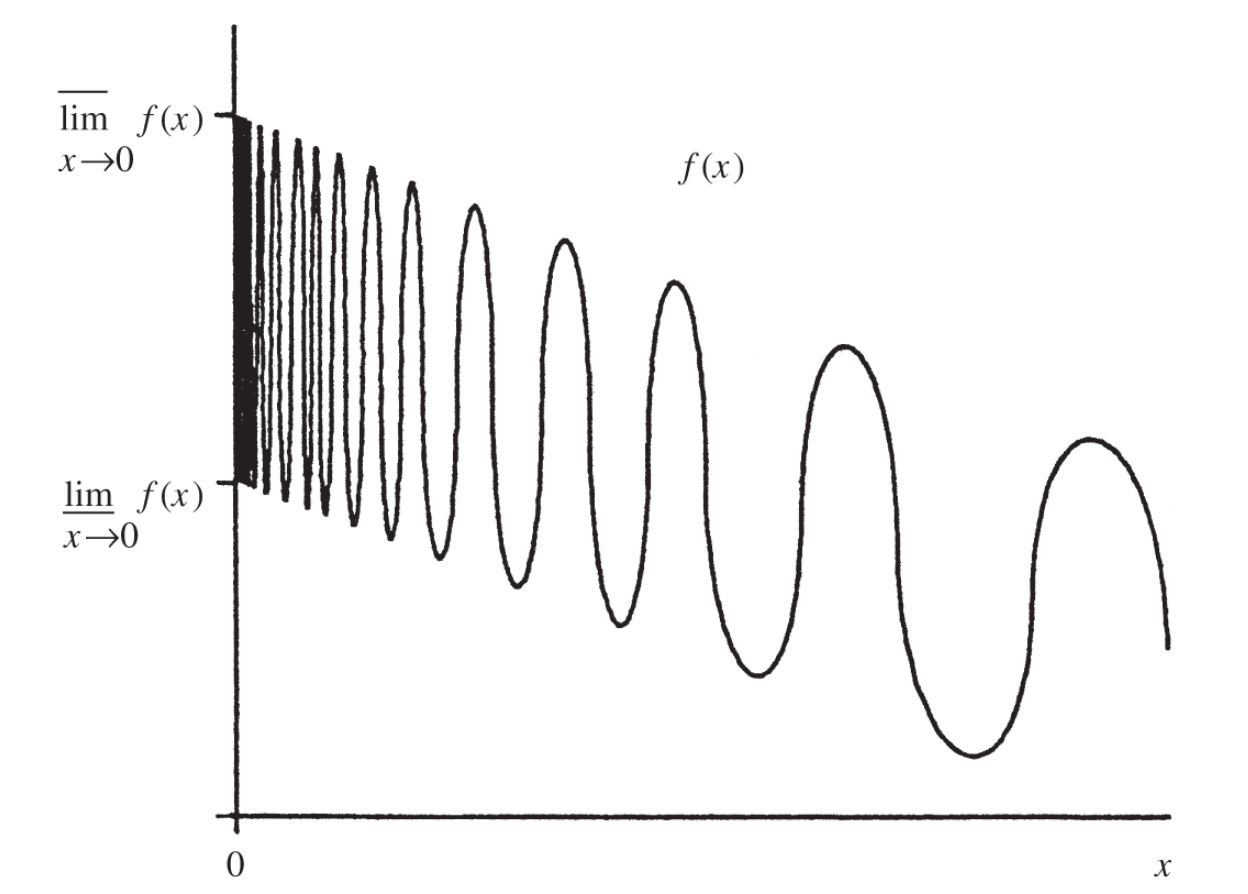
\includegraphics[width=.66\textwidth]{images/limit1.png}
    \caption{The upper and lower limits of a function.}
    \label{fig:lowerupperlimit}
\end{figure}

We write $f(x) \sim g(x)$ to mean that $f(x) / g(x) \rightarrow 1$ as $x \rightarrow 0$.

\begin{theorem}[Lipschitz functions are continuous]\label{LipschitzContinuous}
\end{theorem}

\textit{Proof}: Assum that the function $f: X \rightarrow Y$ is a Lipschitz function s.t. 
$|f(x)-f(y)| \leq c|x-y| (x, y \in X)$ for some constant $c\geq 0$.
Then, $\forall \epsilon > 0$, let $\displaystyle \delta = \frac{\epsilon}{c}$, and we have
$\forall x, y\in X, |x-y| < \delta \Rightarrow \displaystyle |x-y| < \frac{\epsilon}{c} \Rightarrow |f(x) - f(y)| \leq c |x-y| \leq c\cdot \frac{\epsilon}{c} = \epsilon \Rightarrow$ Lipschitz functions are continuous.

\begin{definition}[Homeomorphism]
    If $f: X \rightarrow Y$ is a continuous bijection with continuous 
    inverse $f^{-1}: Y \rightarrow X$, then $f$ is called a homeomorphism, 
    and $X$ and $Y$ are termed homeomorphic sets. 
\end{definition}
\begin{corollary}
    Congruences, similarities 
    and affine transformations on $\mathbb{R}^{n}$ are examples of homeomorphisms.
\end{corollary}

\begin{definition}[Differentiable]
    If $f: \mathbb{R}^{n} \rightarrow \mathbb{R}^{n}$, we say that $f$ is 
    differentiable at $x$ and has derivative given by the linear mapping 
    $f^{\prime}(x): \mathbb{R}^{n} \rightarrow \mathbb{R}^{n}$ if
$$
\lim _{h \rightarrow 0} \frac{\left|f(x+h)-f(x)-f^{\prime}(x) h\right|}{|h|}=0 .
$$
\end{definition}

\begin{definition}[Pointwise Convergence]
    For a sequence of functions: $f_k : X\rightarrow Y$ where $X$ and $Y$ are subsets 
    of Euclidean spaces. $f_k$ converge pointwise to a function $f:X\rightarrow Y$ if 
    $f_k(x)\rightarrow f(x)$ as $k\rightarrow \infty$.
\end{definition}

\begin{definition}[Unifrom Convergence]
    For a sequence of functions: $f_k : X\rightarrow Y$ where $X$ and $Y$ are subsets 
    of Euclidean spaces. $f_k$ converge uniformly to a function $f:X\rightarrow Y$ if 
    $sup_{x\in X} |f_k(x)- f(x)| \rightarrow 0$ as $k\rightarrow \infty$.
\end{definition}

\textbf{Note}: Uniform convergence is a stronger property than pointwise convergence i.e. Uniform convergence implies pointwise convergence, but not the other way around

\begin{definition}[Another Definition of Pointwise Convergence]
For each $x\in D$, $\forall\delta > 0$, $\exists k_{x, \delta}>0$, s.t. whenever $k > k_{x, \delta}$, $|f_k(x)-f(x)| < \delta$.
\end{definition}

\begin{definition}[Another Definition of Uniform Convergence]
$\forall\delta >0$, $\exists k_\delta>0$ s.t. whenever $k>k_\delta$, $|f_k(x) - f(x)|<\delta$.
\end{definition}

\textbf{Note}: the main difference between pointwise and uniform convergence is that pointwise convergence is for each $x$ in the domain, whereas uniform convergence is for all $x$ in domain. And this is also the reason why $\sup$ shown in the definition in the textbook.



\begin{theorem}
    If the functions $f_k$ are continuous and converge uniformly to $f$, then $f$ is continuous. 
\end{theorem}


\begin{theorem}[Logarithms]
    Apparently, $a^c = b^{c\log a / \log b}$
\end{theorem}
